\subsection{Scénario Cockburn}
\textbf{Cas d'utilisation:} Sortir

\textbf{Acteur primaire:}  Le conducteur

\textbf{Pré-condition:} Paiement a été accepté.
 
\textbf{Post-condition:} Le deuxième barriere est abaissée. 

\textbf{Scenario primaire: } \\
    \textbf{1.} La borne change la couleur du feu (vert). \\
    \textbf{2.} La borne léve la deuxième barrière. \\
    \textbf{3.} Le conducteur passe pour la deuxième barriere. \\
    \textbf{4.} Le deuxième boucle detecte si le véhicule est sortie.\\ 
    \textbf{5.} La borne change la couleur du feu (rouge).\\
    \textbf{6.} La borne abaisse la deuxième barrière. \\

\textbf{Variantes:}\\
    \textbf{1a.} Le feu ne change pas de couleur. Donc une alarme est levé vers  l'ordinateur  du  poste de surveillance. \\
    \textbf{2a.}  La deuxième barriere barriere ne se léve pas. Donc une alarme est levé vers  l'ordinateur du poste de surveillance.
    
\newpage    
\subsection{Diagramme d'activité}
\begin{figure}[!htb]
    \centering
    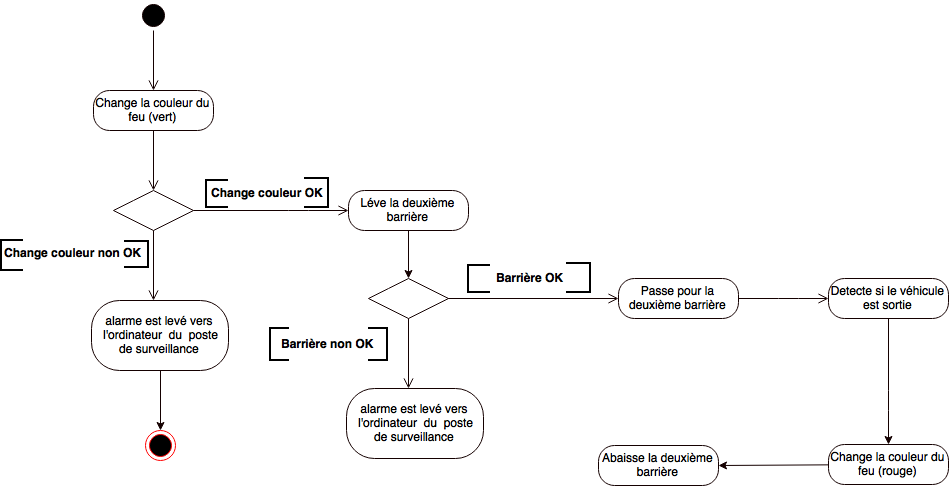
\includegraphics[scale=0.5, angle = 90]{02_Desenvolvimento/TD2/images/DASortir.png}
    \caption{Diagramme d'activité - Sortir}
    \label{fig:DARentrer}
\end{figure}
\newpage    
\subsection{Collaboration}
\begin{figure}[!htb]
    \centering
    %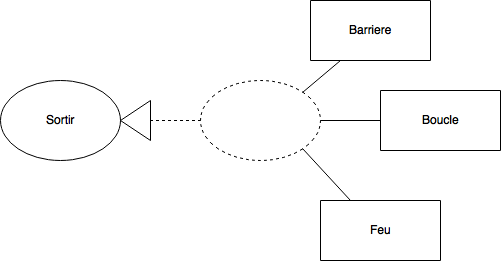
\includegraphics[scale=0.45, angle = 90]{02_Desenvolvimento/TD2/images/ColaSortir.png}
    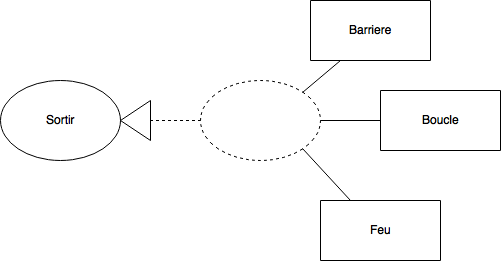
\includegraphics[scale=0.6]{02_Desenvolvimento/TD2/images/ColaSortir.png}
    \caption{Collaboration - Sortir}
    \label{fig:DARentrer}
\end{figure}